\documentclass[letterpaper,12pt]{article}
\usepackage[latin1]{inputenc}
\usepackage[english]{babel}
\usepackage{amssymb,amsmath}
\usepackage[pdftex]{graphicx}
%\usepackage{natbib}
\usepackage{color}
\usepackage{layout}
\usepackage{float}
\hoffset-1.5cm
\voffset-1.5cm
\setlength{\textwidth}{17cm}
\setlength{\textheight}{21.5cm}

\title{Selecci�n de grupo como un mecanismo de evoluci�n de la cooperatividad}
\author{Luis Alejandro Mahecha\\Proyecto de Tesis de Maestria en Ciencias F�sica\\Departamento de F�sica\\Tutor: Juan Manuel Pedraza\\Grupo de Biof�sica\\Universidad de los Andes}
\date{}

\begin{document}
\maketitle
\section{$2\times 2$ Games}
At these games a population of individuals  have pairwise interactions with two behavioral strategies to choose from, the elements of the payoff matrix 
\begin{equation}
\bordermatrix{~ & C & D \cr
             C & R & S \cr
              D & T & P \cr}
\end{equation}
are the parameters of the strategies and determine the dynamics of population, for prisoner's dilemma($T>R>P>S$). There are two ways to simulate these: solving the differential replication equation\footnote{http://www.univie.ac.at/virtuallabs/TwoByTwo/mixed.html}
\begin{equation}
\frac{dx}{dt}=x(x-1)(P_C - P_D)
\end{equation}
 and the stochastic code with a replication probability depending on the average payoff of the two strategies to choose. 
\\
\par
The stochastic code works as follow; a population of $N$ individuals with two strategies $C$(cooperate) and $D$(defect) where $x$ individuals behave as $C$ and $N-x$ as $D$, then the average payoffs respect to whole population for a cooperator and a defector are
\begin{equation}
P_{C}=\frac{R(x-1)+S(N-x)}{N-1}
\end{equation} 
\begin{equation}
P_{D}=\frac{Tx+P(N-x-1)}{N-1}
\end{equation}
 With a population of $N=10000$ and parameters $R=0.4$ $S=0$ $T=0.8$ $P=0.2$. The plots of $P_C$ and $P_D$ as functions of $x$ are
 \begin{figure}[H]
\begin{center}
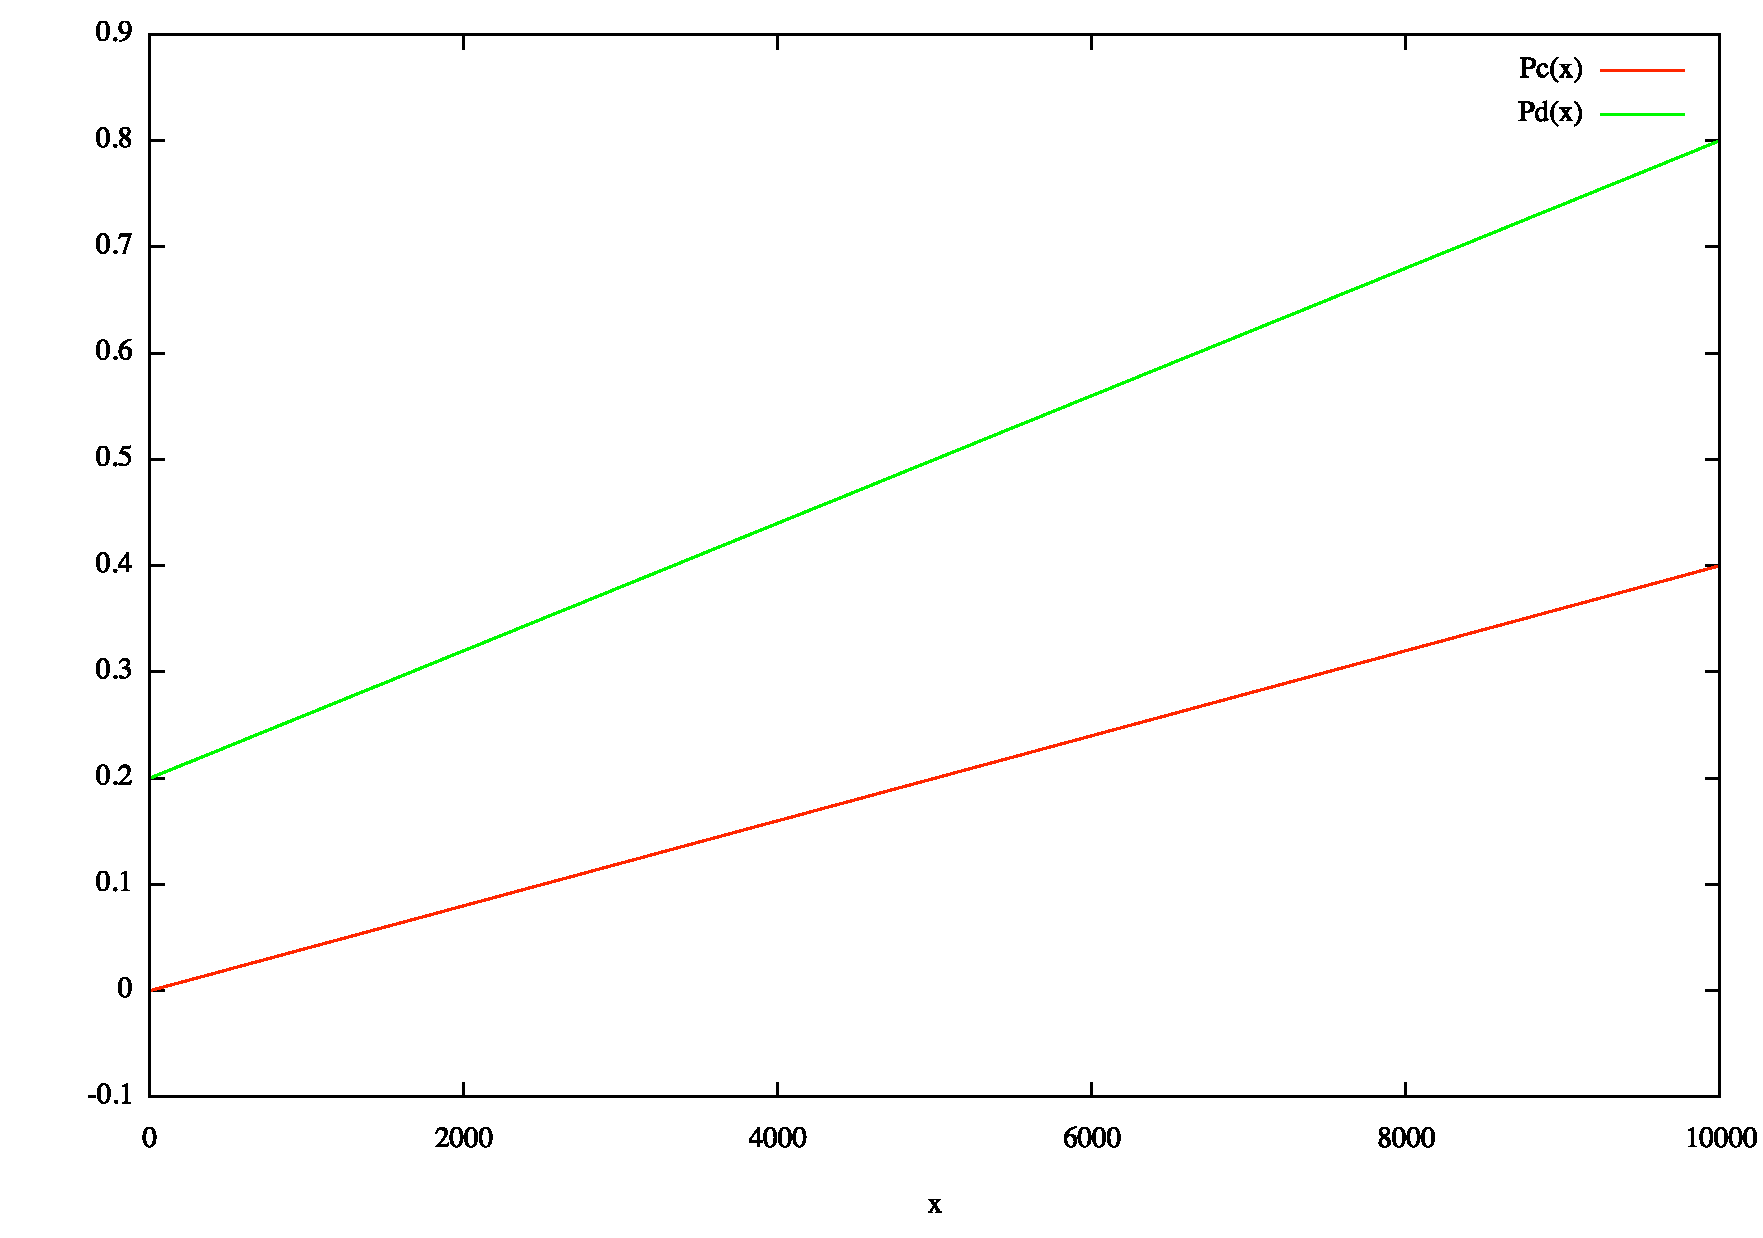
\includegraphics[width=11cm,height=10cm]{PcPd.pdf}
\caption{\footnotesize $P_C$ and $P_D$ payoffs plots}
\end{center}    
\end{figure}
The probability of cooperate $\rho_{c}=P_{C}/(P_{C}+P_{D})$
\begin{figure}[H]
\begin{center}
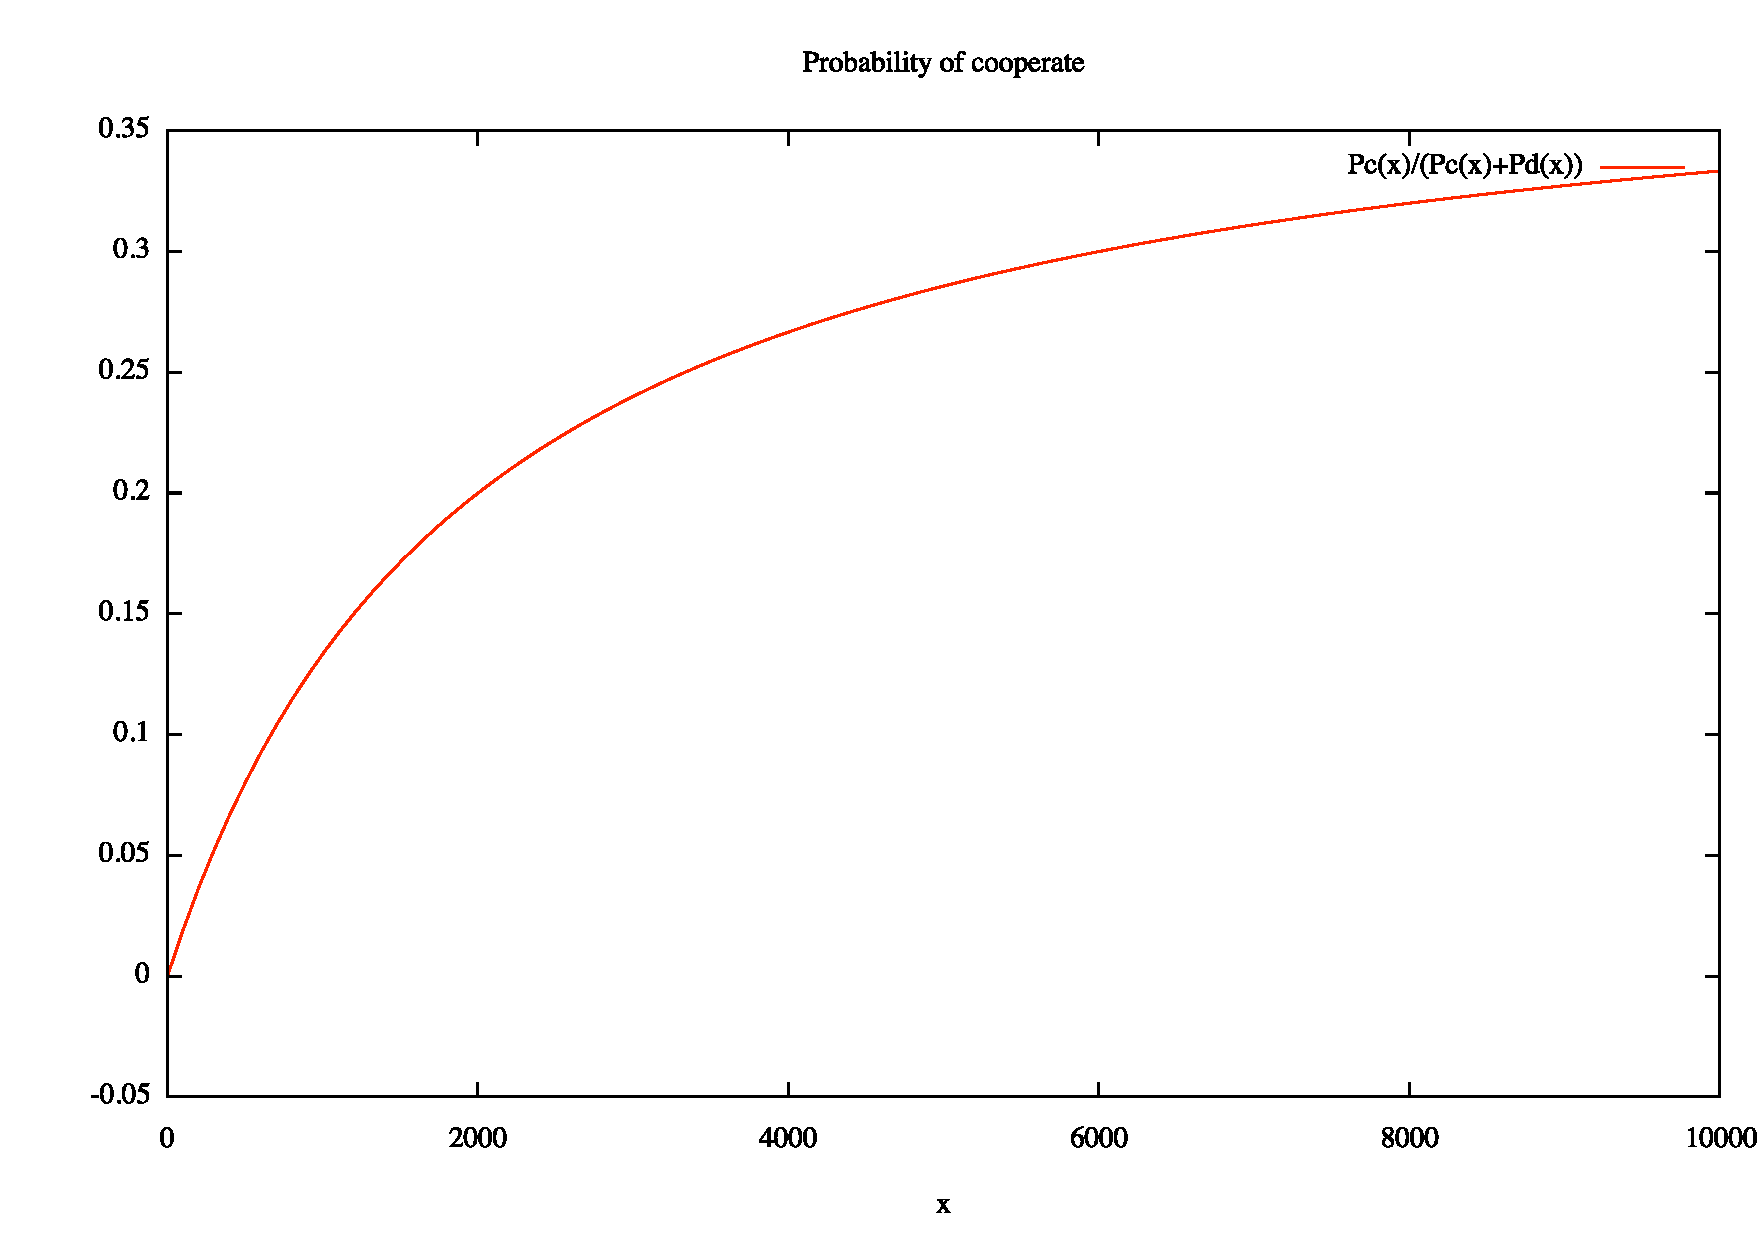
\includegraphics[width=11cm,height=10cm]{probability.pdf}
\caption{\footnotesize Probability $\rho_{c}(x)$ of cooperate}
\end{center}    
\end{figure}
 The next plot was done with a simulation that works as Monte-Carlo step, if a random number in the range $[0,1]$ is less than $\rho_c$ the individual cooperates and stay for next iterations( using only if) even the random number is larger than $\rho_c$.
  \begin{figure}[H]
\begin{center}
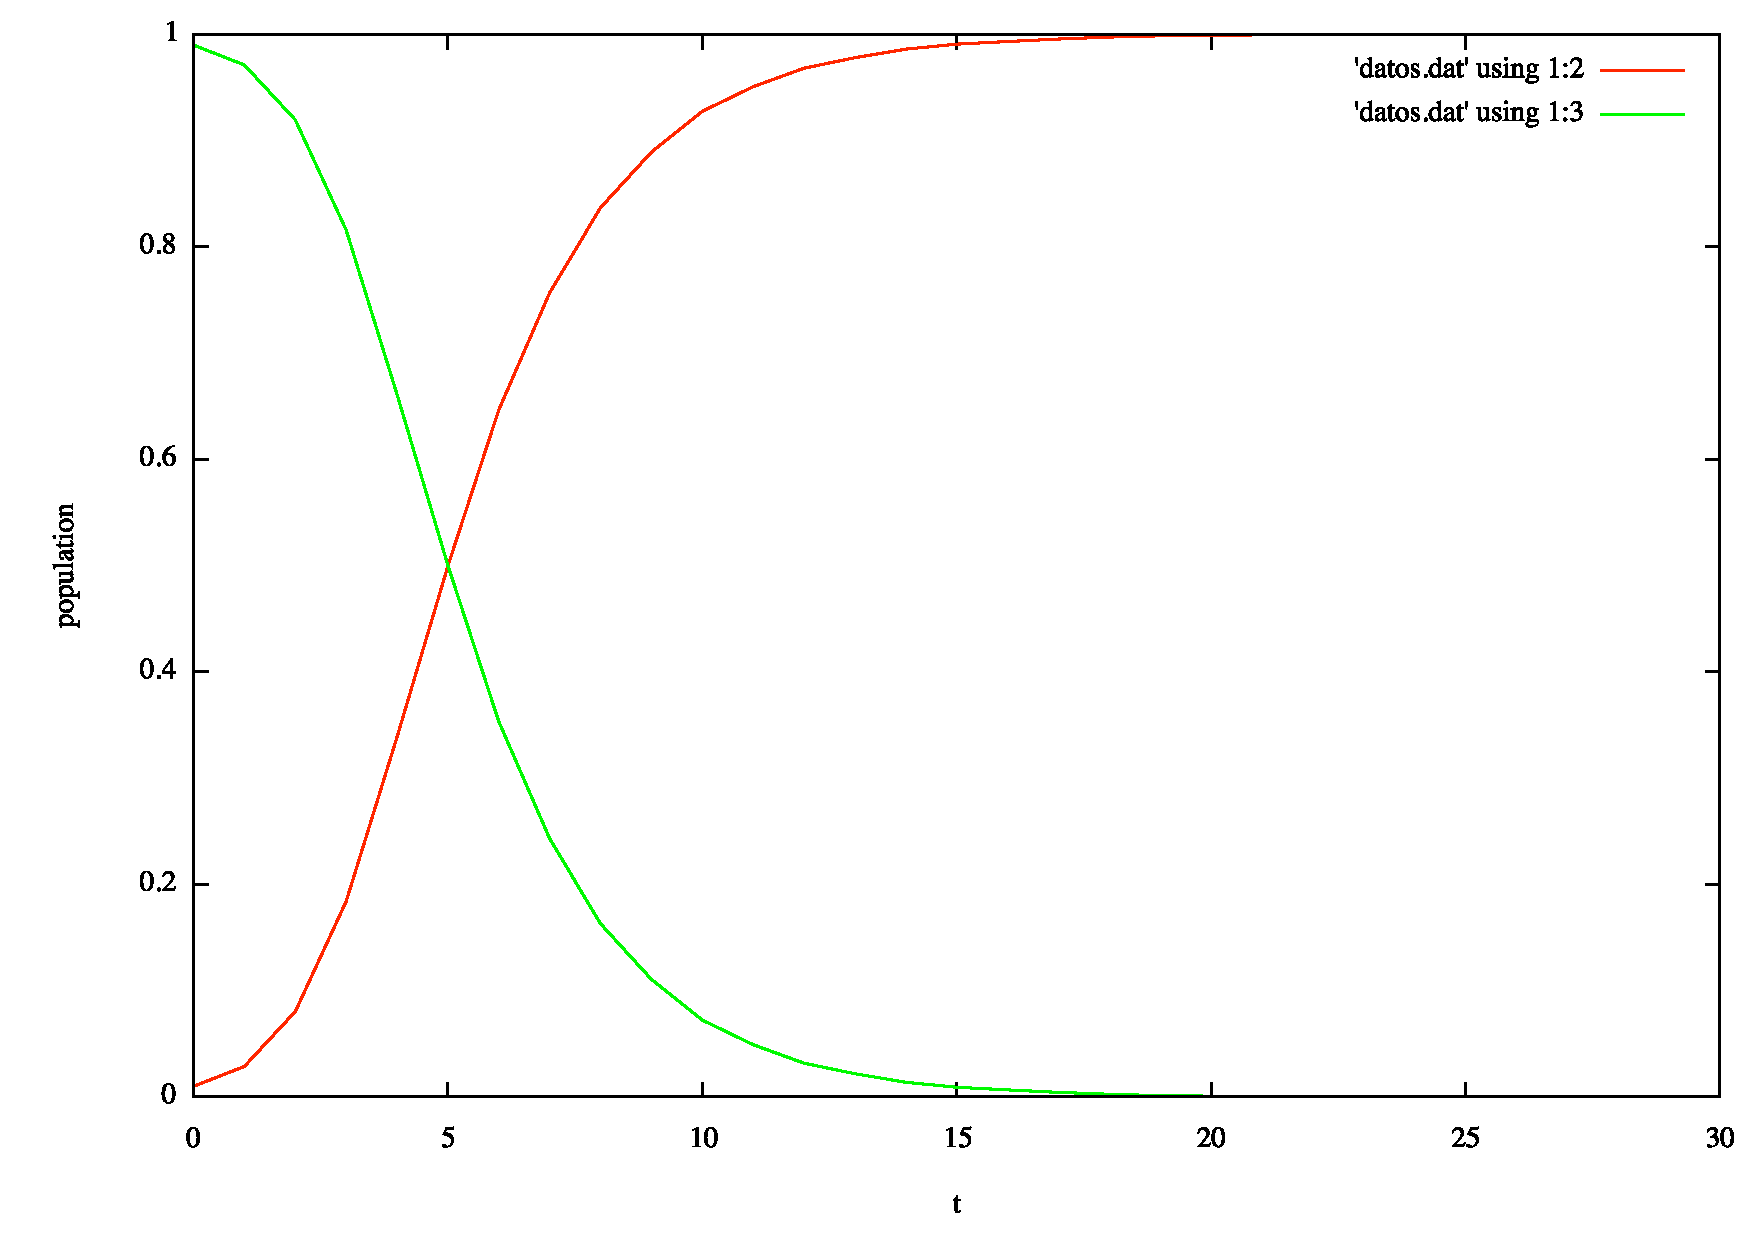
\includegraphics[width=11cm,height=8cm]{prisoners.pdf}
\caption{\footnotesize Red line fraction of cooperators and green line fraction of defectors}
\end{center}    
\end{figure}
Now using parameters $R=1$, $S=0$, $T=0.7$ y $P=0.2$, the expected payoff $P_C$ is less than $P_D$ for low population of cooperators, as show Figure(4).
\begin{figure}[H]
\begin{center}
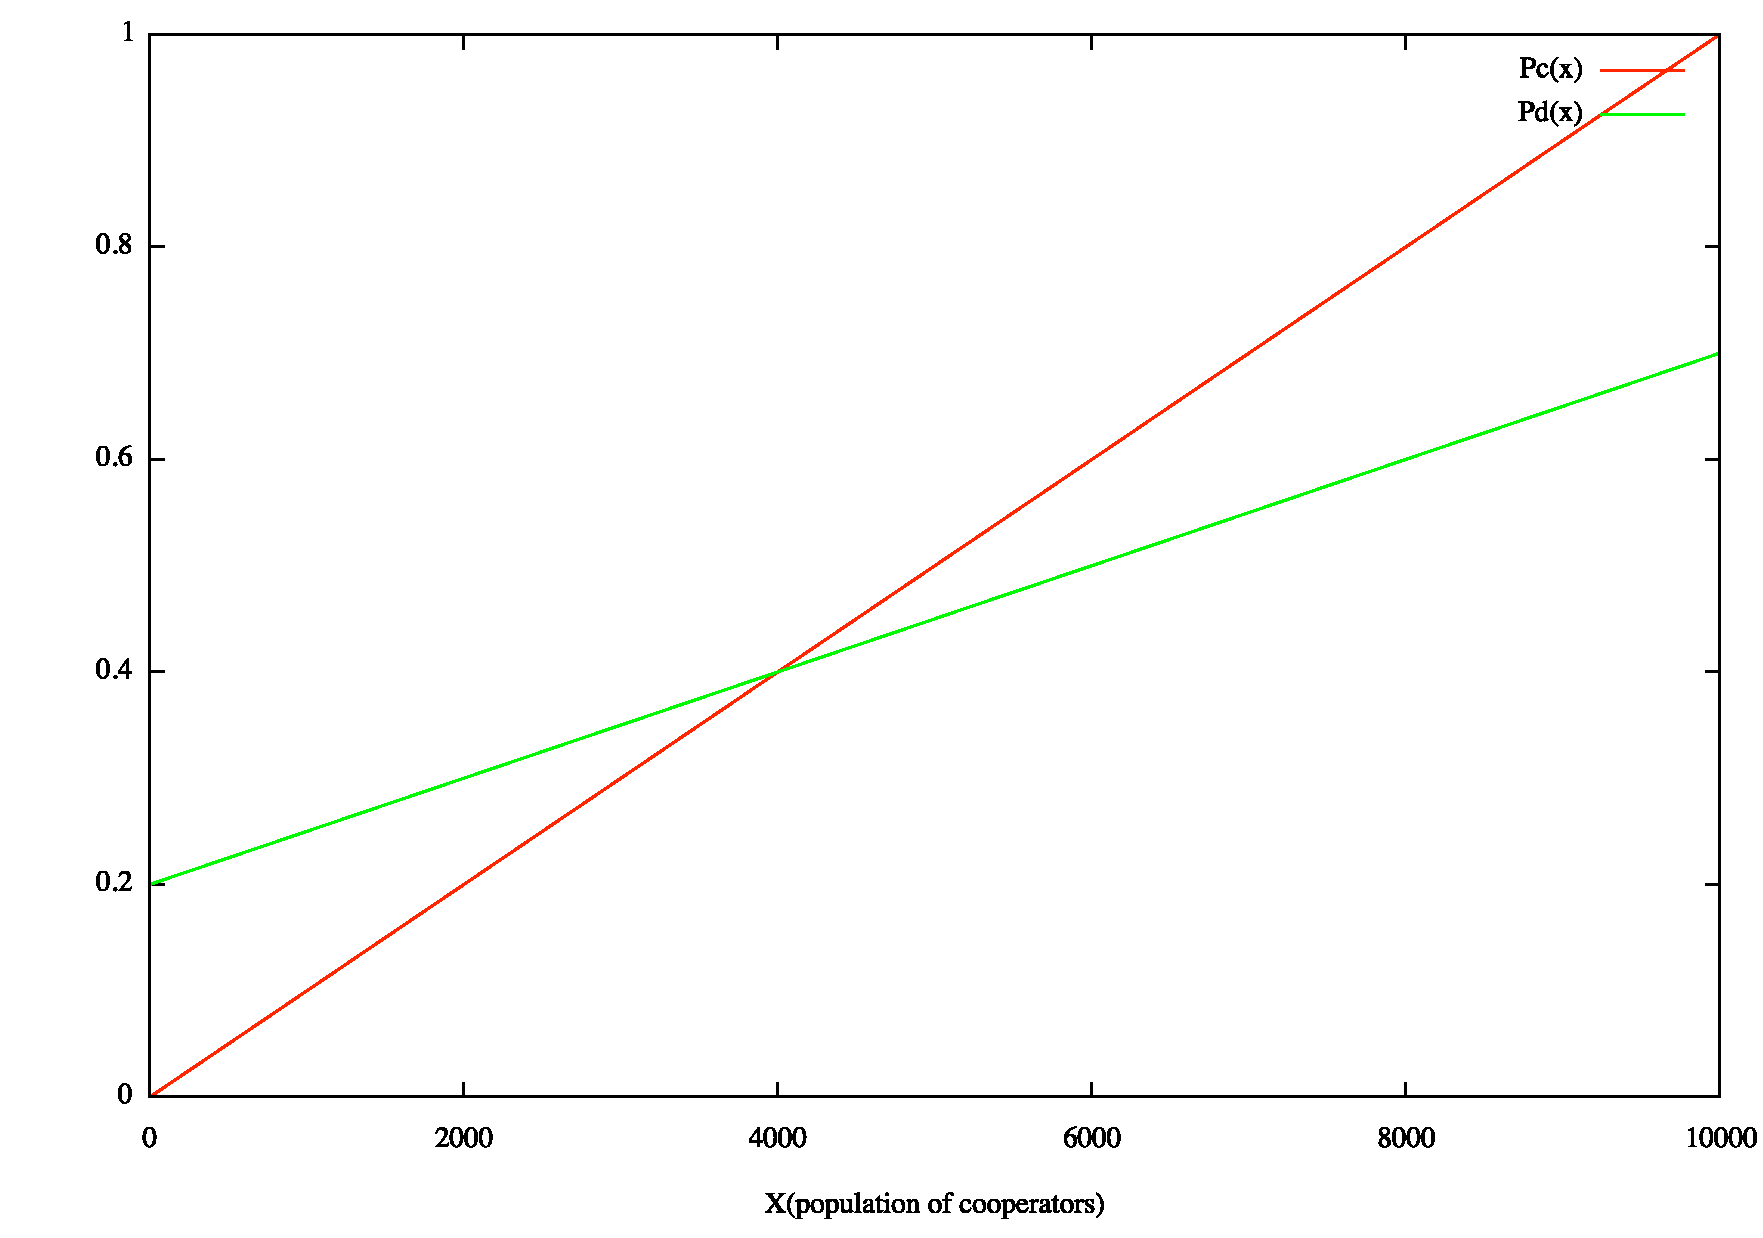
\includegraphics[width=11cm,height=8cm]{p2.pdf}
\caption{\footnotesize Plots of payoff $P_C$ and $P_D$}
\end{center}    
\end{figure}
This time the probability for the stochastic process is proportional to the payoffs difference 
\begin{equation}
\rho_c=\frac{1}{2} + \frac{(P_C - P_D)}{2MAX_{P_C - P_D}}
\end{equation}  
where $MAX_{P_C - P_D}$ is the highest difference $P_C - P_D$. Including the parameter $0\leq w\leq 1$ that controls the intensity of selection:
\begin{equation}
\rho_c=\frac{1}{2} + \frac{w(P_C - P_D)}{2MAX_{P_C - P_D}}
\end{equation}  
 For $w=1$ and probability of change for next iterations(using if and else) the result of the simulation was
 \begin{figure}[H]
\begin{center}
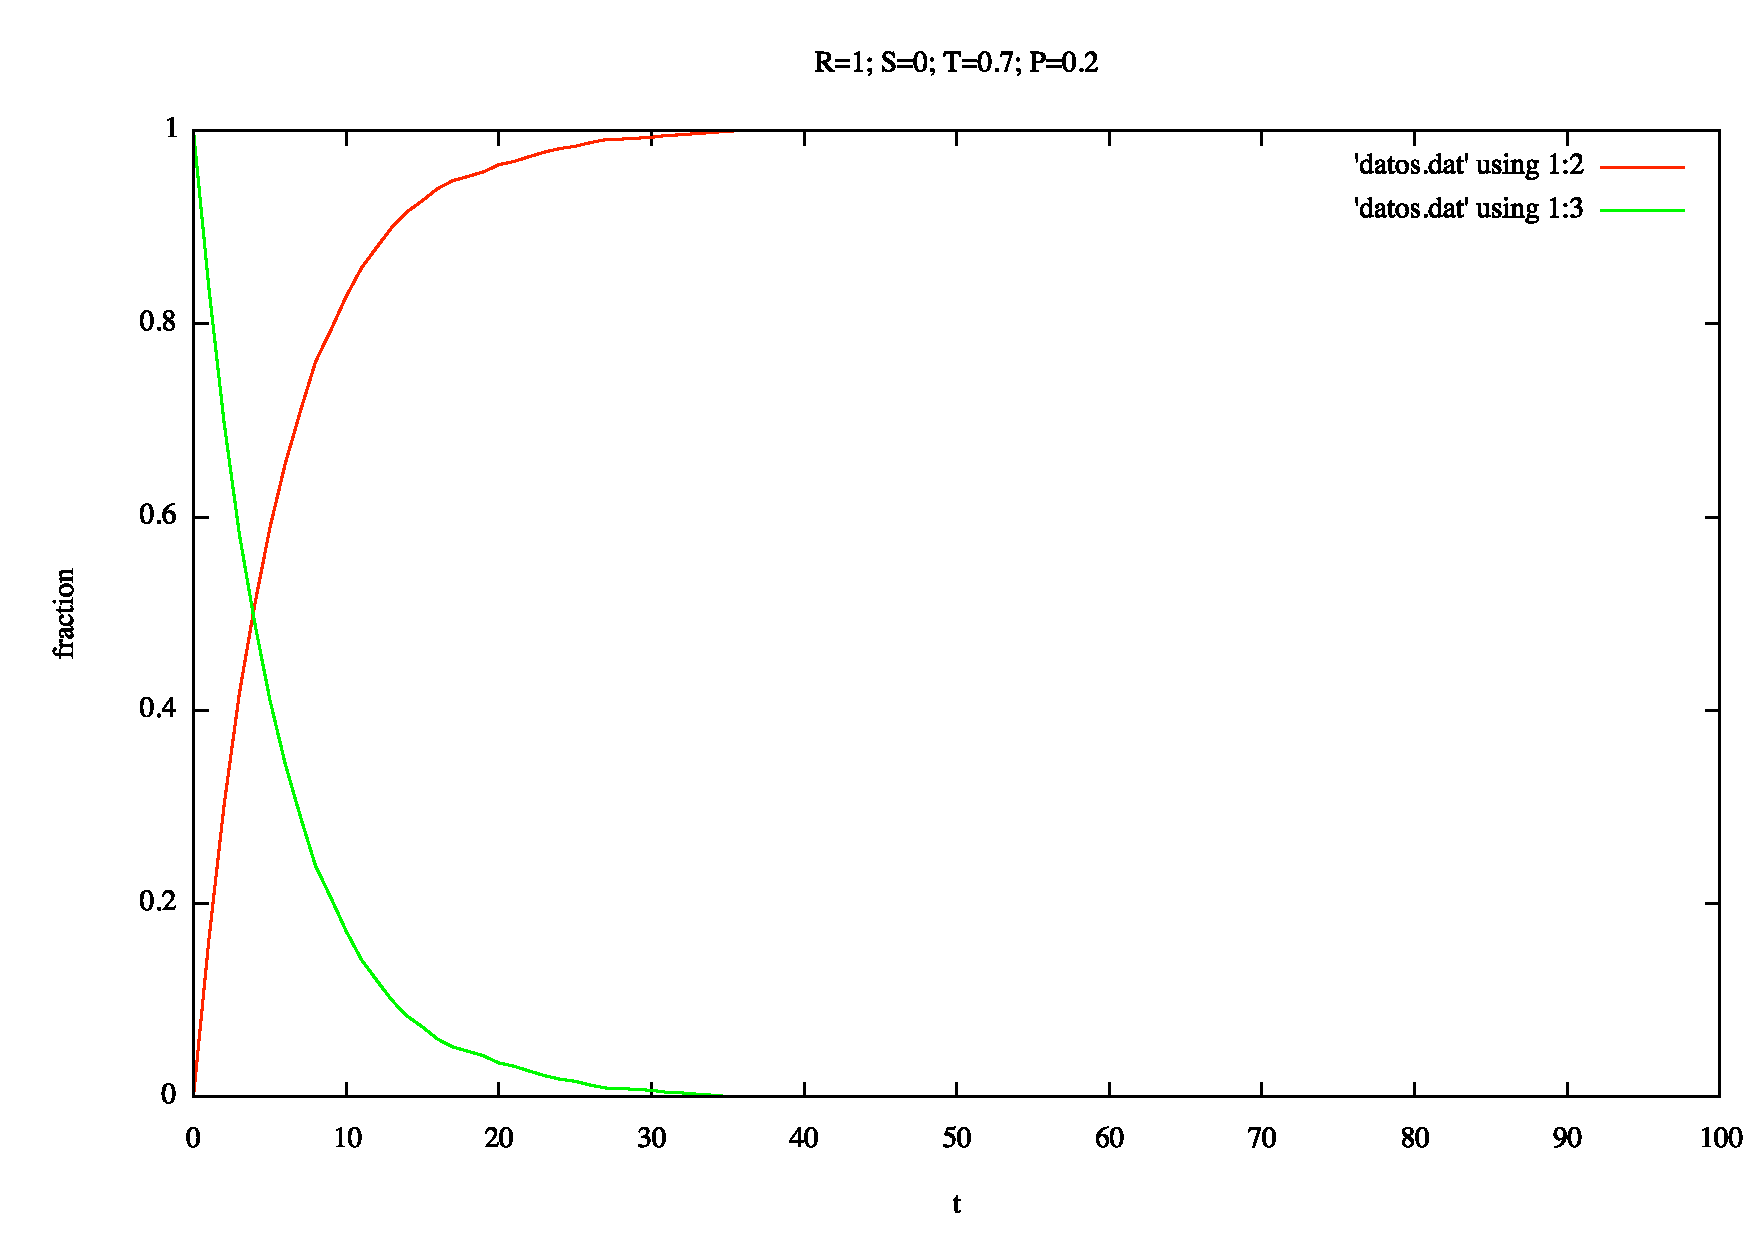
\includegraphics[width=11cm,height=8cm]{dilema2.pdf}
\caption{\footnotesize Red line fraction of cooperators and green one fraction of defectors}
\end{center}    
\end{figure}
\section{Replicator Dynamics: Moran process}
In the Moran process, at each time step one individual of the population is chosen randomly for reproduction, with a probability that depends of its fitness, the new offspring replaces other individual of the population that is chosen randomly. The fitness and probability functions can be implemented in several forms, the fitness is usually a lineal function  or an exponential function of the expected payoff and the probability is a function of the difference strategies fitness or the fraction of the total payoff.\par
The next simulation is the basic Moran process where an individual is chosen for reproduction using an uniform random generator and other random individual is replaced by the new offspring. The total number of individuals $n$ is fixed and has two types: individuals $0$ and $1$, the number of $1$ individuals is denoted by $i$. The simulation start whit the initial condition $i>0$ and stops when one of the two types dominates the population, randomly some times type $1$ dominate and others type $0$.
\begin{figure}[H]
\begin{center}
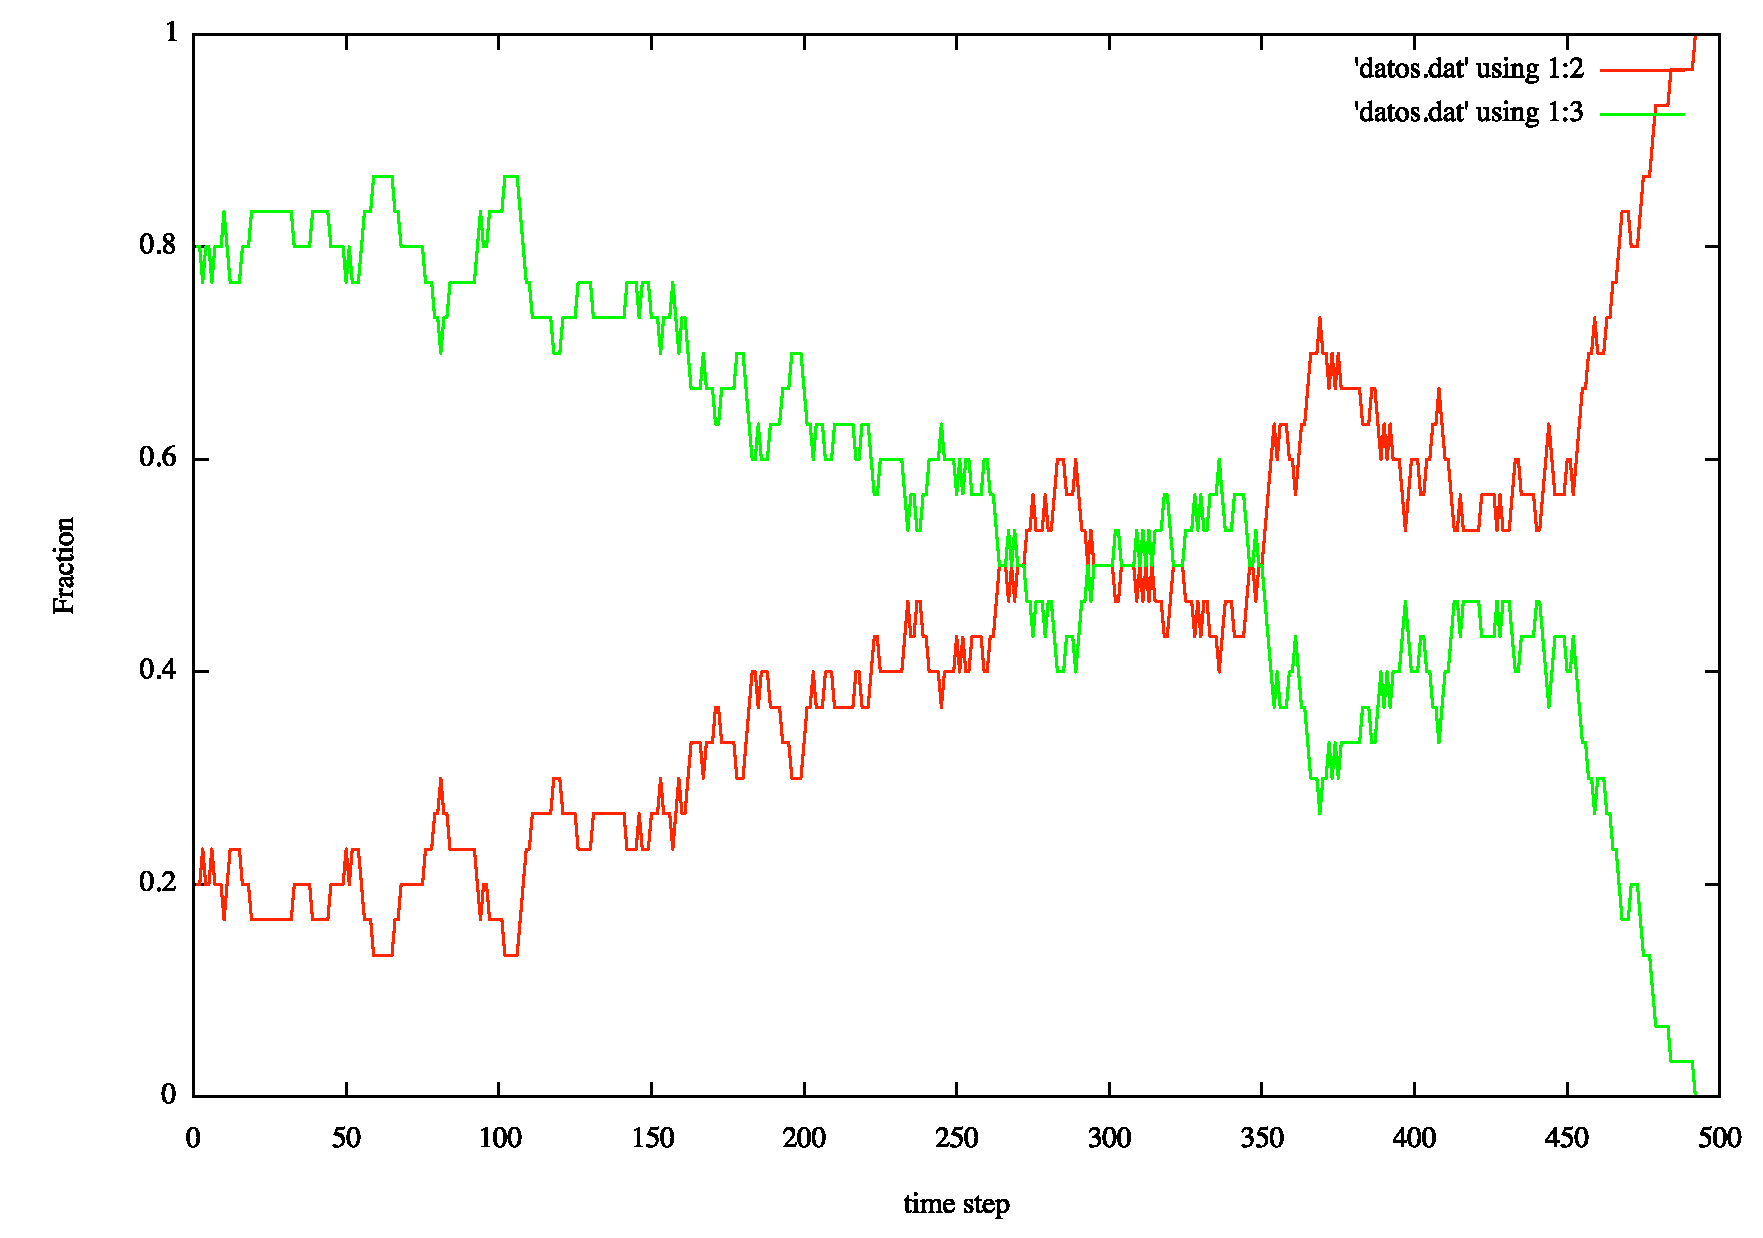
\includegraphics[width=10cm,height=7cm]{bmoran.pdf}
\caption{\footnotesize Red line fraction of type $1$ and green one fraction of type $0$, first round(this was obtained with Basicmoran.cpp).}
\end{center}    
\end{figure}
\begin{figure}[H]
\begin{center}
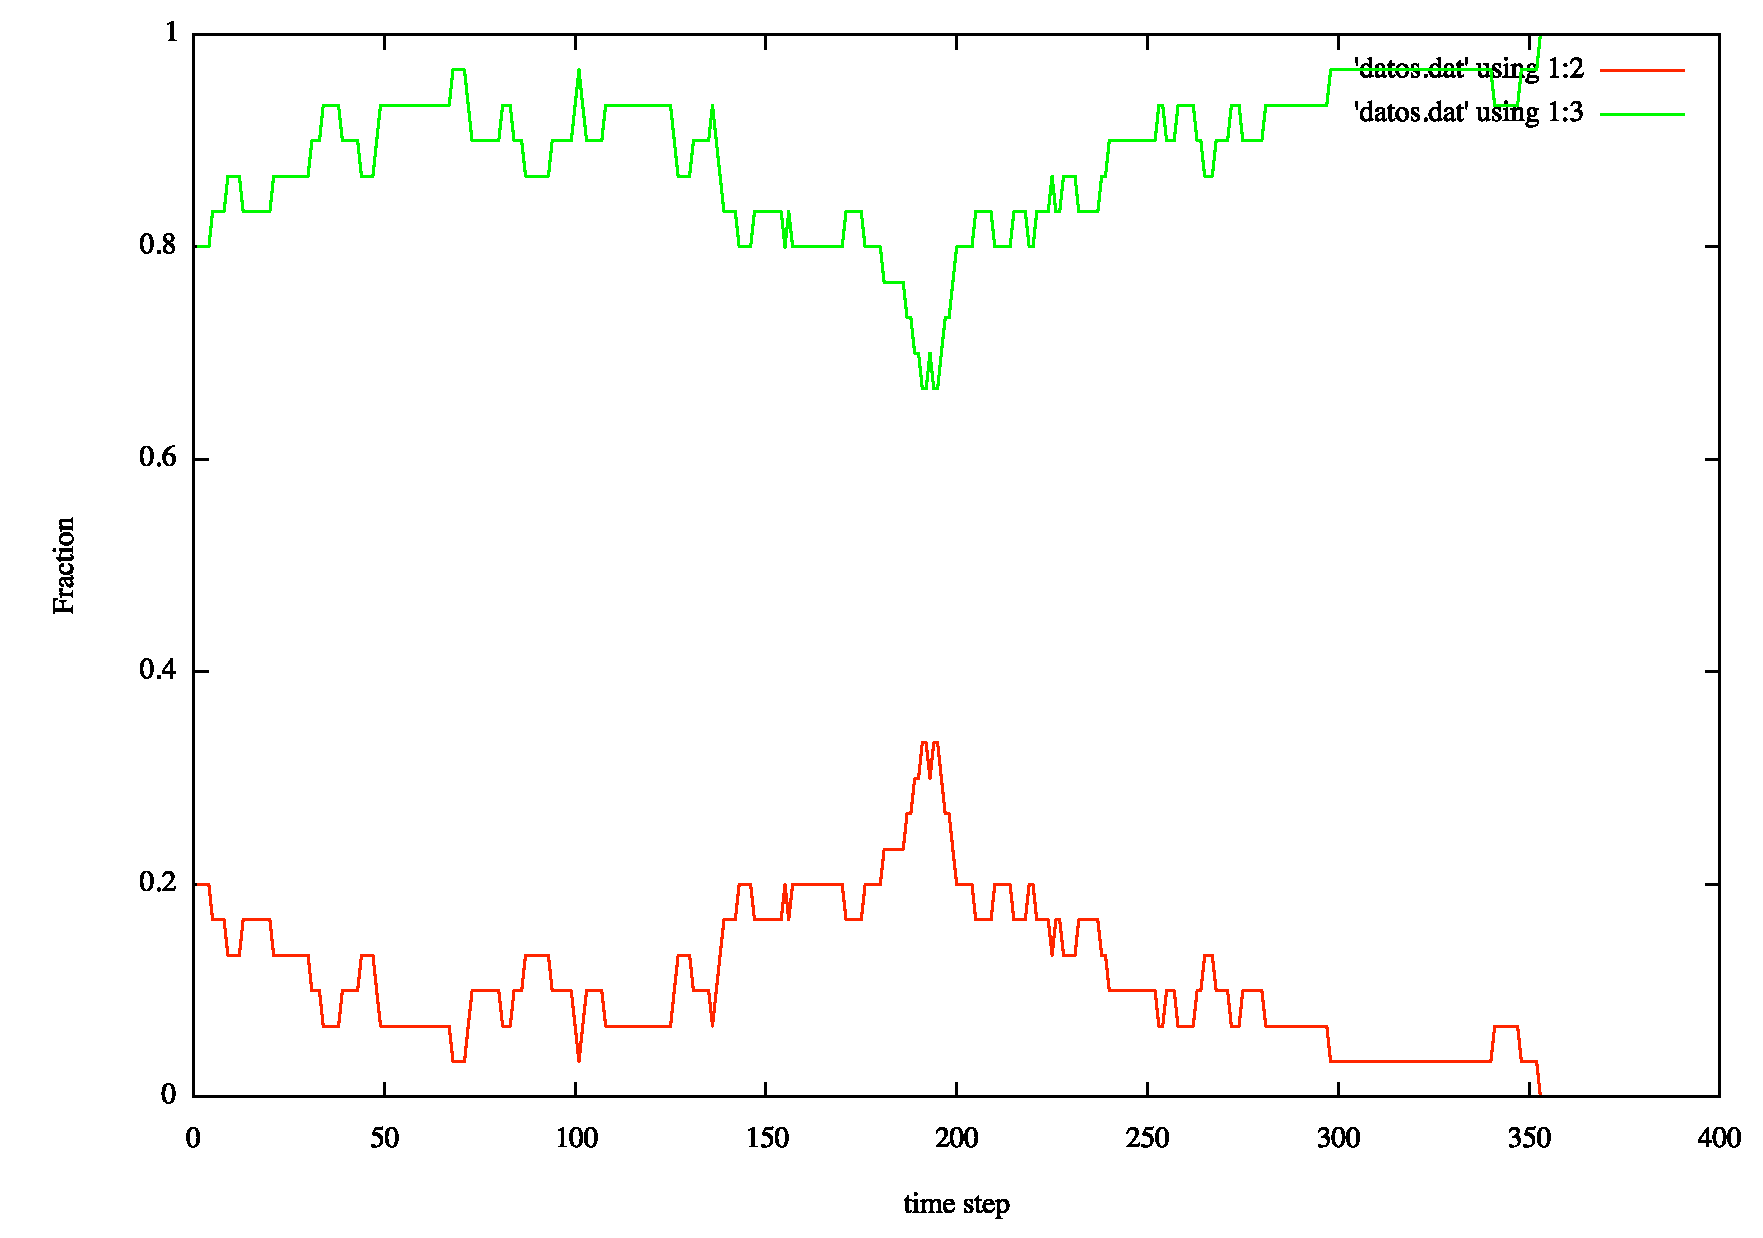
\includegraphics[width=10cm,height=7cm]{bmoran1.pdf}
\caption{\footnotesize second round(this was obtained with Basicmoran.cpp).}
\end{center}    
\end{figure}
The analytical development  to find the probability of dominance is as follow. Whit a population of size $n$ and $i$ individuals of type $1$, the probabilities of choosing are: $i/n$ for type $1$ and $(n-i)/n$ for type $0$. Then the probability  that the population changes from $i$  to $i+1$ is 
\begin{equation}
p_{i,i+1}=\frac{i(n-i)}{n^2},
\end{equation}   
and from $i$ to $i+1$ is
\begin{equation}
p_{i,i-1}=\frac{(n-i)i}{n^2}.
\end{equation}
 The probability $\rho_i$ of fixation or dominance for the initial condition of $i$ individuals of type $1$, is $\rho_i=0$ if $i=0$ and $\rho_i=1$ if $i=n$, this is because of when an individual is chosen to dead it is replaced by one of its same type. The probability $\rho_i$ is the sum of the probabilities of dominate from three events, that is
 \begin{equation}
 \rho_i=p_{i,i}\rho_i + p_{i,i-1}\rho_{i-1} + p_{i,i+1}\rho_{i+1} \;\;\;\; i=1, 2, 3, ..., n-1
 \end{equation}  
 deafening the new variables
 \begin{equation*}
 y_i= \rho_{i}-\rho_{i-1}
  \end{equation*}
  The series of $y_i$ is a geometric series
\begin{equation}
\sum_{i=1}^{n}y_i=\rho_{n}-\rho_{0}=1.
\end{equation} 
Since $p_{i,i-1}=p_{i,i+1}$ and $p_{i,i}=1-2p_{i,i+1}$, let us write equation (9) as
\begin{equation*}
\rho_{i}2p_{i,i+1}=p_{i,i+1}(\rho_{i-1}+\rho_{i+1})
\end{equation*}
\begin{equation}
\rho_{i}-\rho_{i-1}=\rho_{i+1}-\rho_{i}
\end{equation}
because $\rho_0 = 0$, them $y_i=\rho_1$ and $\sum_{i=1}^{n}y_i=\rho_{n}-\rho_{0}=n\rho_{1}$. To determine $\rho_i$ note that $\rho_i = \sum_{j=1}^{i}y_j =i\rho_1$, them finally
\begin{equation}
\rho_{i}=\frac{i}{n}.
\end{equation} 
We can perform the same calculation for the same process as before but assuming that type $1$ has fitness $r$ and type $0$ fitness $1$. Them the probability that $1$ is chosen for reproduction is
\begin{equation}
\frac{ri}{ir+n-i}
\end{equation}
that $1$ is chosen for elimination is
\begin{equation}
\frac{i}{n}.
\end{equation}
Type $0$ has probability for reproduction $n-i/(ri+n-i)$ and $n-i/n$ for elimination. Therefore the probabilities of transition are
\begin{equation}
p_{i,i+1}=\frac{ri}{ri+n-i}\frac{n-i}{n}
\end{equation}
\begin{equation}
p_{i,i-1}=\frac{n-i}{ri+n-i}\frac{i}{n}
\end{equation}
\begin{equation}
p_{i,i}=1-p_{i,i+1}-p_{i,i-1}.
\end{equation}
Ones again the conditions for fixation probabilities $\rho_{i}$ are $\rho_{0}=0$, $\rho_{n}=1$ and
\begin{equation}
\rho_{i}=p_{i,i}\rho_{i}+p_{i,i+1}\rho_{i+1}+p_{i,i-1}\rho_{i-1}.
\end{equation}
 With the new variable $y_{i}=\rho_{i}-\rho_{i-1}$ we can write equation (18) as
 \begin{equation}
 y_i = y_{i+1}\frac{p_{i,i+1}}{p_{i,i-1}}=y_{i+1}\frac{ri}{n-i}\frac{n-i}{i}
 \end{equation}
 them $y_{i+1}=\frac{1}{r}y_i$, and these lead to
\begin{equation}
y_i =\frac{1}{r^{i-1}}\rho_1
\end{equation}  
since $1=\rho_1 (1+\sum_{m=1}^{n-1}\frac{1}{r^{m}} )$ and $\rho_i=\rho_1 (1+\sum_{j=1}^{i-1}\frac{1}{r^{j}} )$, the fixation probability is
\begin{equation}
\rho_{i}=\frac{1+\sum_{j=1}^{i-1}\frac{1}{r^j}}{1+\sum_{m=1}^{n-1}\frac{1}{r^m}}.
\end{equation}
In this expression we have telescopic series. The sum value for a telescopic series is
\begin{equation}
\sum_{i=0}^{n}\frac{1}{x^n}=\frac{1-\frac{1}{x^{n+1}}}{1-\frac{1}{x}}.
\end{equation}  
Therefore the probability of fixation for type $1$ starting in state $i$ is
\begin{equation}
\rho_i = \frac{1-1/r^i}{1-1/r^n}.
\end{equation}

This result can be checked in a Moran process simulation where is measured  the fixation probability as a function of $r$. In the figure below are showed the analytical curve and the stochastic measures.
\begin{figure}[H]
\begin{center}
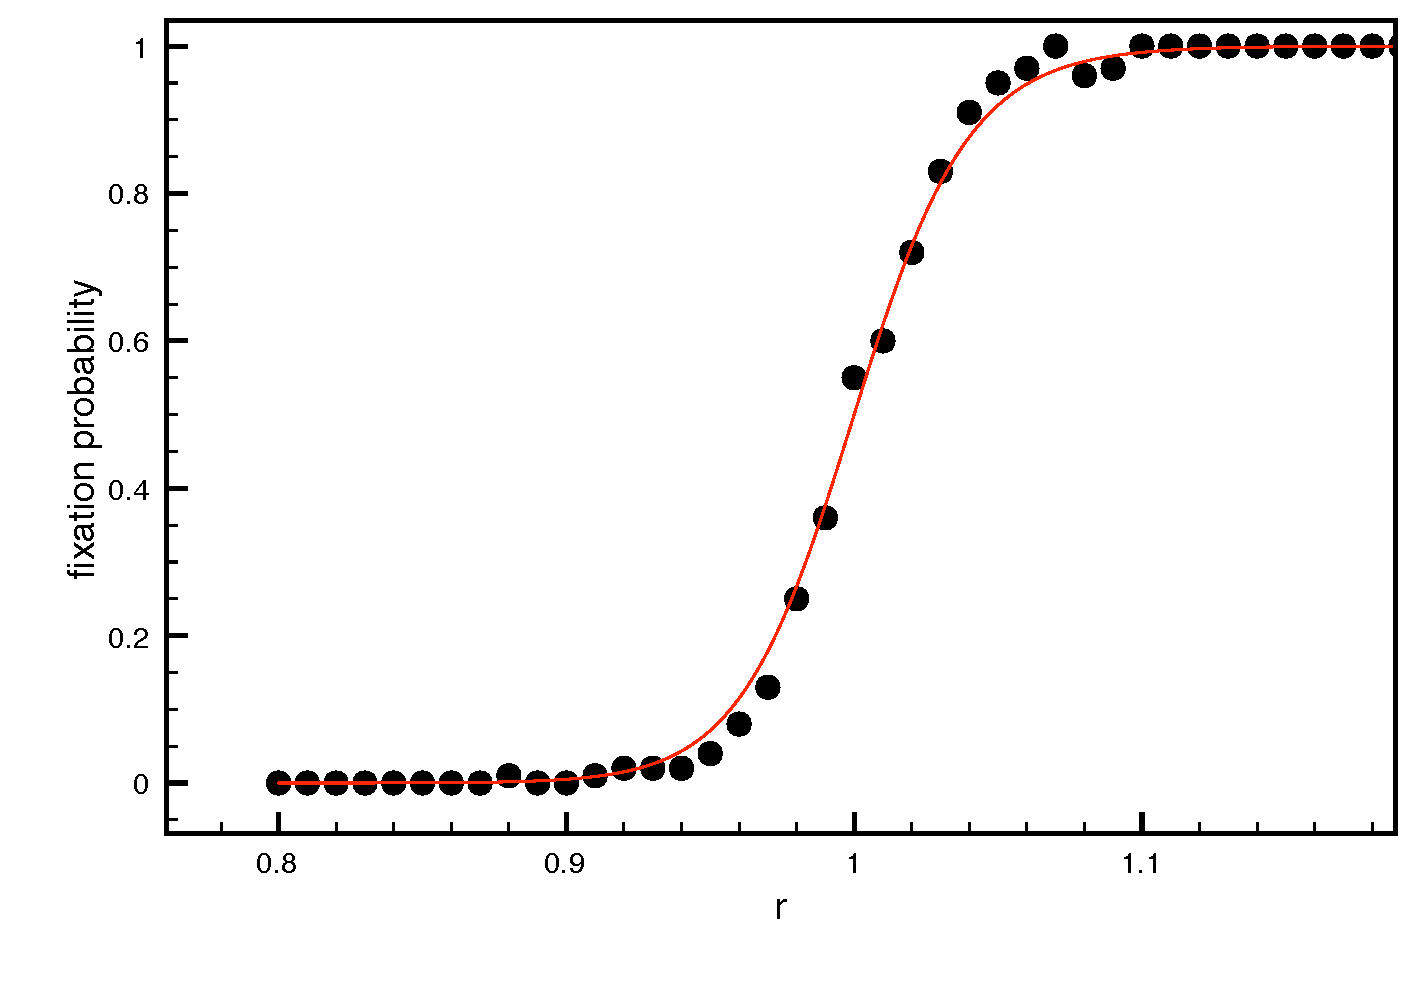
\includegraphics[width=10cm,height=7cm]{plot.pdf}
\caption{\footnotesize Red line, plot of equation (23) with $i=50$ and $n=100$, black points represent the stochastic simulation (this was obtained with RamdonDriftbucle.cpp).}
\end{center}    
\end{figure}
In the next figure there is a plot of $	\rho_i$ as a function of $i$, which shows that the probability $\rho_i$ is $1$ for values of $i$ greater than $6$.
\begin{figure}[H]
\begin{center}
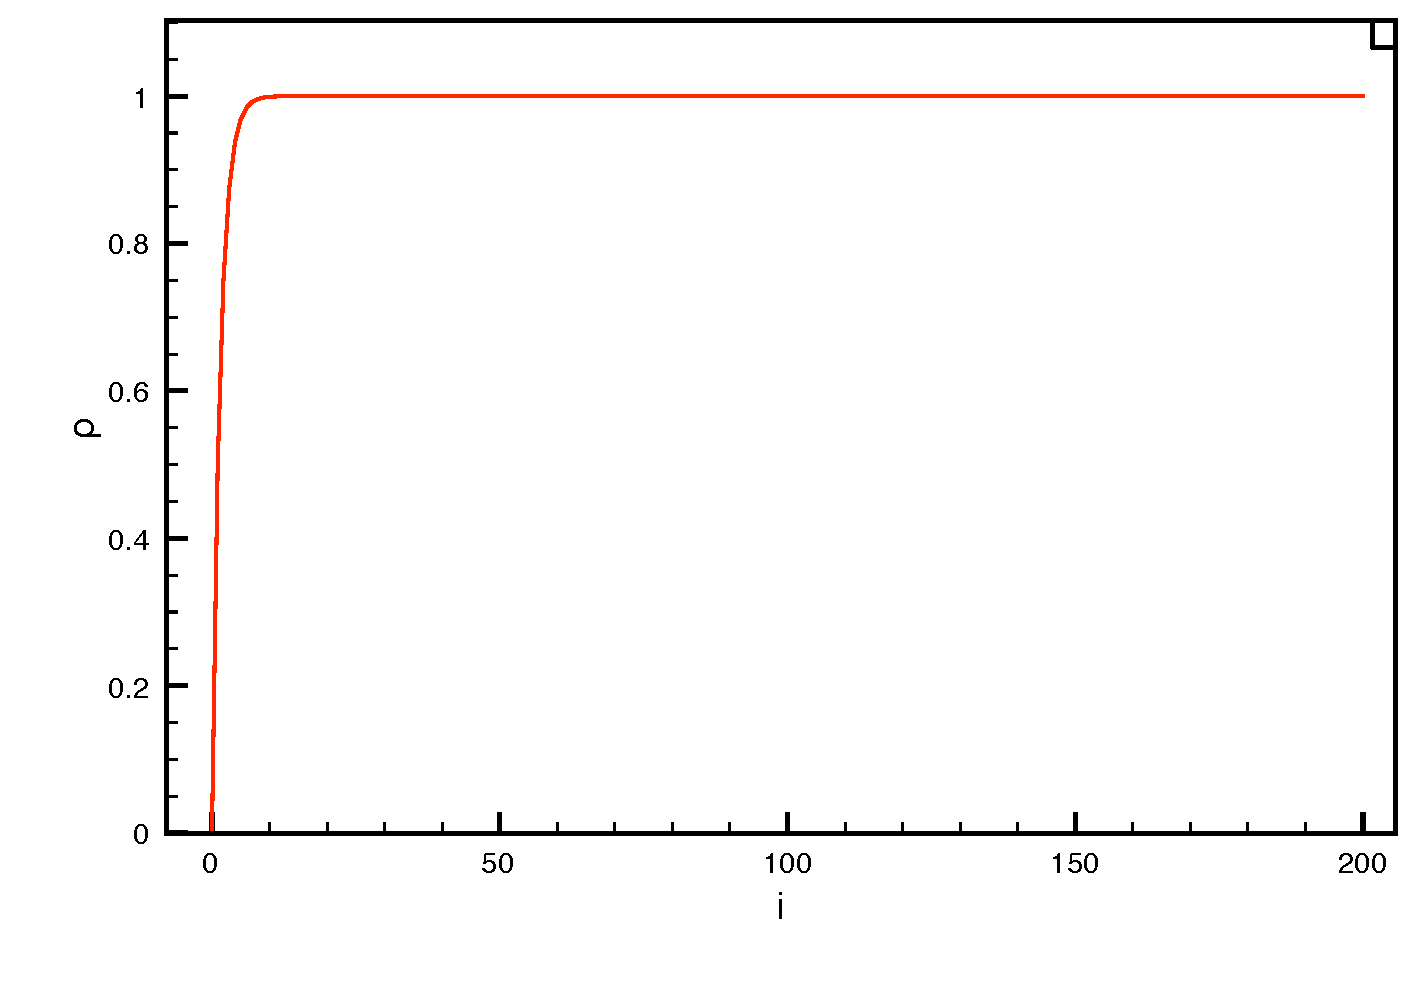
\includegraphics[width=10cm,height=7cm]{populationi1000.pdf}
\caption{\footnotesize Plot of $\rho_i$ with $n=1000$ and $r=2$.}
\end{center}    
\end{figure}
Assuming alleles with fitness $r$ and $s$, the transition probabilities become
\begin{equation}
\begin{split}
P_{i,i+1}&=\frac{ri}{ri+s(n-i)}\frac{n-i}{n}\\
P_{i,i-1}&=\frac{s(n-i)}{ri+s(n-i)}\frac{i}{n}
\end{split}
\end{equation} 
replacing into the recurrence equation for $y_{i}$
\begin{equation}
y_{i+1}=y_{i}\frac{s}{r}
\end{equation}
which leads to
\begin{align}
\nonumber y_{i}= \left( \frac{s}{r}\right)^{i-1}\rho_{1},\\
\rho_{1}=\frac{1-\left( \frac{s}{r}\right)^{i}}{1-\left( \frac{s}{r}\right)^{n}}
\end{align}
\section{Features to make the simulation closer to the experiment conditions and real world}
 An spacial array with next neighbors and a distribution of fitness for each allele, for this work it is going to be implemented the distribution of fitness which is doing by giving several possible  values of fitness to each allele. Then the initial condition will be a gaussian distribution for the individuals of each type of allele. It is known that the phenotype variability of an allele is due to the noise in the expression of its gene and which leads to phenotypes that can share value fitness for different alleles.\\
In this model model the fitness for the initial populations of the alleles and their offsprings come from a distribution which can be usually gaussian or poisson's, but by simplicity, initially we are going to use the Gaussian distribution.  
\begin{figure}[H]
\begin{center}
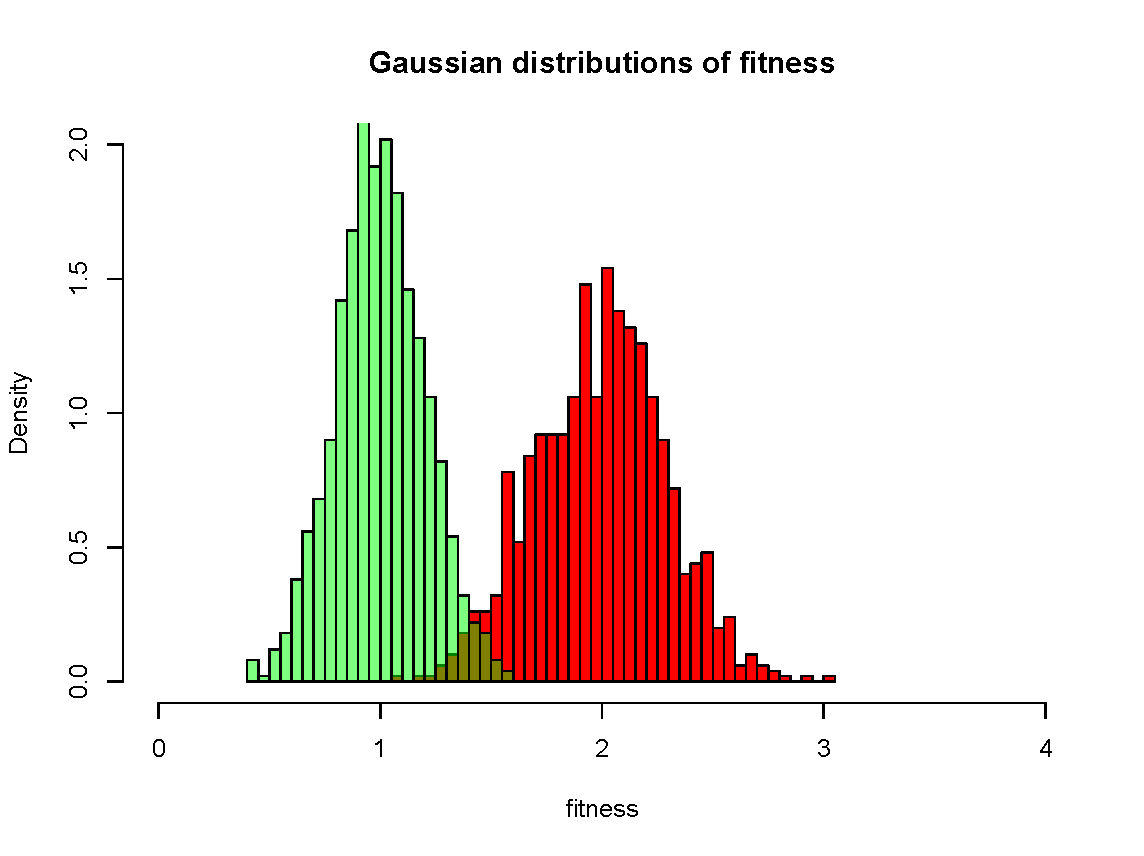
\includegraphics[width=10cm,height=7cm]{alelos.pdf}
\caption{\footnotesize In these figure there is an example where two different alleles produce equals values of fitness }
\end{center}    
\end{figure}
Let individuals of alleles of types $1$ and $0$ have values of fitness $f_{1i}$ and $f0j$ respectibily. Then the probability that type $1$ is choosing for reproduction is
\begin{equation}
p_{reproduction}=\frac{\sum_{i=1}^{n}f_{1i}}{\sum_{i=1}^{n}f_{1i} + \sum_{j=1}^{N-n}f_{0j}}
\end{equation} 
where $n$ is the initial population of type $1$ and $N$ the size of total population. Therefore the probabilities of transition are
\begin{equation}
P_{n,n+1}=\frac{\sum_{i=1}^{n}f_{1i}}{\sum_{i=1}^{n}f_{1i} + \sum_{j=1}^{N-n}f_{0j}}\frac{N-n}{N}
\end{equation}
\begin{equation}
P_{n,n-1}=\frac{\sum_{j=1}^{N-n}f_{0j}}{\sum_{i=1}^{n}f_{1i} + \sum_{j=1}^{N-n}f_{0j}}\frac{n}{N}
\end{equation}
replacing them in equation
\begin{equation*}
y_{n}=y_{n+1}\frac{P_{n,n+1}}{P_{n,n-1}}
\end{equation*}
leads to
\begin{equation}
y_{n}=y_{n+1}\frac{N-n}{n}\frac{\sum\limits_{i=1}^{n}f_{1i}}{ \sum\limits_{j=1}^{N-n}f_{0j}}
\end{equation}
since $y_1=\rho_1$, evaluating (31) for $n=1,2$ gives 
\begin{equation}
\begin{split}
y_2 &=\frac{\rho_1}{N-1}\frac{\sum\limits_{m=1}^{N-1}s_{m}}{\sum\limits_{m=1}^{1}r_{m}},\\
y_3 &=\frac{\rho_1}{N-1}\frac{\sum\limits_{m=1}^{N-1}s_{m}}{\sum\limits_{m=1}^{1}r_{m}}\frac{2}{N-2}\frac{\sum\limits_{m=1}^{N-2}s_{m}}{\sum\limits_{m=1}^{2}r_{m}}
\end{split}
\end{equation}
then by induction 
\begin{equation}
y_{i}=\rho_1\frac{(i-1)!(N-i)!}{(N-1)!}\prod\limits_{j=2}^{i}{\frac{\sum\limits_{m=1}^{N-(j-1)}s_m}{\sum\limits_{m=1}^{j-1}r_m}},\;\;\;\; i\geq 2
\end{equation}
from the condition $\sum_{n=1}^{N}{y_n}$ can be obtained $\rho_1$
\begin{equation}
1=\rho_1 + \sum\limits_{i=2}^{N}{\rho_1\frac{(i-1)!(N-i)!}{(N-1)!}\prod\limits_{j=2}^{i}{\frac{\sum\limits_{m=1}^{N-(j-1)}s_m}{\sum\limits_{m=1}^{j-1}r_m}}}
\end{equation}
\begin{equation}
\rho_1=\left(1 + \sum\limits_{i=2}^{N}{\frac{(i-1)!(N-i)!}{(N-1)!}\prod\limits_{j=2}^{i}{\frac{\sum\limits_{m=1}^{N-(j-1)}s_m}{\sum\limits_{m=1}^{j-1}r_m}}}\right)^{-1}
\end{equation}
In the simulation the time of getting the half of population is similar in both situations: the population with discrete value of fitness and with values from a gauss distribution of fitness figure(11).
\begin{figure}[H]
\begin{center}
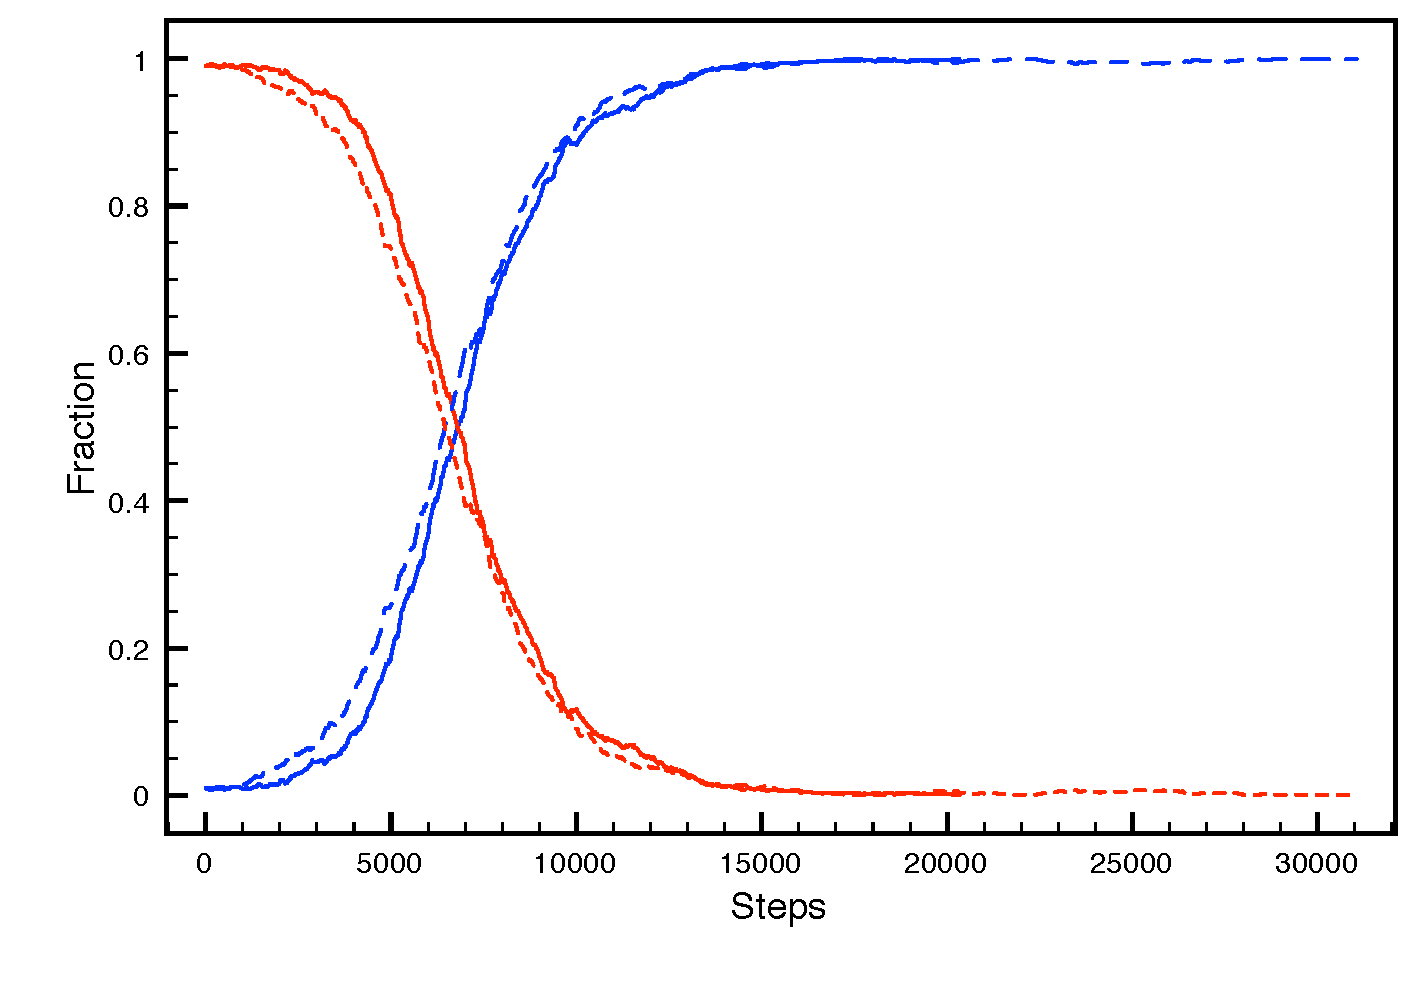
\includegraphics[width=10cm,height=7cm]{DiscretDiss.pdf}
\caption{\footnotesize The dashed lines are the population with discrete fitness while the continued lines with gauss distribution fitness. The discrete population has the next parameters $r=2$ and$s=1$, and the parameters for the gaussian distribution are $r_{pro}=2$, $s_{pro}=1$, $\sigma_{r}=0.3$ and $\sigma_{s}=0.25$. }
\end{center}    
\end{figure}

\bibliographystyle{plain}
\bibliography{cooperation}
%\end{thebibliography}{}
\end{document}

